\documentclass[a4paper]{article}

\usepackage[a4paper,  margin=0.4in]{geometry}
% \usepackage[left=2.5cm,top=3cm,right=2.5cm,bottom=3cm,bindingoffset=0.5cm]{geometry}

\usepackage{graphicx}
\usepackage{float}
\usepackage{hyperref}
\usepackage{multicol}


\usepackage[utf8]{inputenc}
\begin{document}

% \begin{titlepage}
\title{SNR classes project - birds species recognition using deep neural networks
- second stage report}

\author{Michał Sypetkowski, Marcin Lew}
\twocolumn
\maketitle


\section{General information}
Git repository:\newline
\url{https://github.com/msypetkowski/SNR-proj.git}.\newline
Previous stage report: \newline
\url{https://github.com/msypetkowski/SNR-proj/blob/master/doc/main.pdf}.

In all experiments we use Adam optimizer and we exponentially
decrease learning rate by 50\% for 1000 iterations.
We use batch size of 128.

\section{Establishing Layers count}
\label{expLayer}

First, we experiment with layers count.
    We trained 3 different models (they have respectively 11, 8 and 6 layers).
Detailed layers descriptions for each model are shown in tables respectively
\ref{table:layers11},
\ref{table:layers8} and
\ref{table:layers6}.
Rounded total trainable parameters count is respectively: 2.0M, 1.7M  and 1.5M.

Batch normalization with relu activation layers are used in all these models,
where the horizontal lines occur in the tables.

\begin{table}[!hbt]
    \caption{ 11 layer convolutional NN architcture
    \label{table:layers11}
    }
\begin{center}
    \begin{tabular}{| l | l | l | l |}
    \hline
        Layer & kernel/window& strides & output shape\\
    \hline
        Conv1  & (5, 5)&        (1, 1)&     224x224x64  \\
    \hline
        MaxPool1 & (2, 2)&      (2, 2)&     112x112x64  \\
        Conv2  & (5, 5)&        (1, 1)&     112x112x64  \\
    \hline
        MaxPool2 & (2, 2)&      (2, 2)&     56x56x64    \\
        Conv3  & (5, 5)&        (1, 1)&     56x56x64    \\
    \hline
        MaxPool3 & (2, 2)&      (2, 2)&     28x28x64    \\
        Conv4  & (5, 5)&        (1, 1)&     28x28x64  \\
    \hline
        MaxPool4 & (2, 2)&      (2, 2)&     14x14x64  \\
        Conv5  & (5, 5)&        (1, 1)&     14x14x64  \\ % additional
    \hline
        MaxPool5 & (2, 2)&      (1, 1)&     14x14x64  \\
        Conv6  & (5, 5)&        (1, 1)&     14x14x64  \\
    \hline
        MaxPool6 & (2, 2)&      (2, 2)&     7x7x64  \\
        Conv7  & (5, 5)&        (1, 1)&     7x7x64  \\  % additional
    \hline
        MaxPool7 & (2, 2)&      (1, 1)&     7x7x64  \\
        Conv8  & (3, 3)&        (1, 1)&     7x7x128\\
    \hline
        MaxPool8 & (2, 2)&      (2, 2)&     4x4x128  \\
        Conv9  & (2, 2)&        (1, 1)&     4x4x128)\\
    \hline
        MaxPool9 & (2, 2)&      (1, 1)&     4x4x128  \\
        Conv10 & (2, 2)&        (1, 1)&     4x4x128)\\  % additional
    \hline
        MaxPool10 & (2, 2)&      (1, 1)&     4x4x128  \\
        Conv11 & (3, 2)&        (1, 1)&     4x4x128)\\  % 4x4
    \hline
        MaxPool11 & (2, 2)&      (1, 1)&     4x4x128  \\
        Flatten & - & - & 2048 \\
        Dense1 & - & - & 512 \\
    \hline
        Output & - & - & 50 \\
        Softmax & - & - & 50 \\
    \hline
    \end{tabular}
\end{center}
\end{table}

\begin{table}[!hbt]
    \caption{ 8 layer convolutional NN architcture (layer names correspond to some layers names in 11 layer architecture \ref{table:layers11})
    \label{table:layers8}
    }
\begin{center}
    \begin{tabular}{| l | l | l | l |}
    \hline
        Layer & kernel/window& strides & output shape\\
    \hline
        Conv1  & (5, 5)&        (1, 1)&     224x224x64  \\
    \hline
        MaxPool1 & (2, 2)&      (2, 2)&     112x112x64  \\
        Conv2  & (5, 5)&        (1, 1)&     112x112x64  \\
    \hline
        MaxPool2 & (2, 2)&      (2, 2)&     56x56x64    \\
        Conv3  & (5, 5)&        (1, 1)&     56x56x64    \\
    \hline
        MaxPool3 & (2, 2)&      (2, 2)&     28x28x64    \\
        Conv4  & (5, 5)&        (1, 1)&     28x28x64  \\
    \hline
        MaxPool4 & (2, 2)&      (2, 2)&     14x14x64  \\
        Conv6  & (5, 5)&        (1, 1)&     14x14x64  \\
    \hline
        MaxPool6 & (2, 2)&      (2, 2)&     7x7x64  \\
        Conv8  & (3, 3)&        (1, 1)&     7x7x128\\
    \hline
        MaxPool8 & (2, 2)&      (2, 2)&     4x4x128  \\
        Conv9  & (2, 2)&        (1, 1)&     4x4x128)\\
    \hline
        MaxPool9 & (2, 2)&      (1, 1)&     4x4x128  \\
        Conv11 & (3, 2)&        (1, 1)&     4x4x128)\\  % 4x4
    \hline
        MaxPool11 & (2, 2)&      (1, 1)&     4x4x128  \\
        Flatten & - & - & 2048 \\
        Dense1 & - & - & 512 \\
    \hline
        Output & - & - & 50 \\
        Softmax & - & - & 50 \\
    \hline
    \end{tabular}
\end{center}
\end{table}



\begin{table}[!hbt]
    \caption{ 6 layer convolutional NN architcture (layer names correspond to some layers names in 11 layer architecture \ref{table:layers11})
    \label{table:layers6}
    }
\begin{center}
    \begin{tabular}{| l | l | l | l |}
    \hline
        Layer & kernel/window& strides & output shape\\
    \hline
        Conv1  & (5, 5)&        (1, 1)&     224x224x64  \\
    \hline
        MaxPool1 & (2, 2)&      (2, 2)&     112x112x64  \\
        Conv2  & (5, 5)&        (1, 1)&     112x112x64  \\
    \hline
        MaxPool2 & (2, 2)&      (2, 2)&     56x56x64    \\
        Conv3  & (5, 5)&        (1, 1)&     56x56x64    \\
    \hline
        MaxPool3 & (4, 4)&      (4, 4)&     28x28x64    \\
        Conv6  & (5, 5)&        (1, 1)&     14x14x64  \\
    \hline
        MaxPool6 & (2, 2)&      (2, 2)&     7x7x64  \\
        Conv8  & (3, 3)&        (1, 1)&     7x7x128\\
    \hline
        MaxPool8 & (2, 2)&      (2, 2)&     4x4x128  \\
        Conv11 & (3, 2)&        (1, 1)&     4x4x128)\\  % 4x4
    \hline
        MaxPool11 & (2, 2)&      (1, 1)&     4x4x128  \\
        Flatten & - & - & 2048 \\
        Dense1 & - & - & 512 \\
    \hline
        Output & - & - & 50 \\
        Softmax & - & - & 50 \\
    \hline
    \end{tabular}
\end{center}
\end{table}

\subsection{Results}
We use coross entropy as a loss function.
We train each model for 5K iterations with initial learning rate of 0.03.
Accuracy curves are shown in figure \ref{fig:layersAcc}.

Training accuracy increases faster for models with fewer layers.
Smaller networks naturally learn faster, but they have fewer degrees of freedom
and may get worse results in the end.
11-layer network architecture shown to be too complicated for
our dataset and/or training method.
Best accuracy was achieved by medium -- 8-layer network.
We use this architecture for further experiments.

\begin{figure}[!hbt]
    \centering
    \includegraphics[page=2,width=0.5\textwidth]{curvesLayers.png}
    \label{fig:layersAcc}
    \caption[]{Accuracy curves for models with different layers count}
\end{figure}

\section{Experiments with last convolutional layer size}

Our 8-layer network from section \ref{expLayer}, outputs
feature vectors of size 2048 from the last (see Conv11 in table \ref{table:layers8}) convolutional layer (after flattening).
We tried models with 1024 and 4096 sizes of these vectors.
The results are shown are shown in figure \ref{fig:lastSize}.
These dimensions significiantly affect total trainable parameters count
(around 11M in case of 1024 dimensions and around 28M in case of 4096 dimensions).
Decreasing or increasing this parameter caused only loss in accuracy
(models have in the end not enough or too many parameters for our dataset).
% 1024 1138674
% 4096 2810226

\begin{figure}[!hbt]
    \centering
    \includegraphics[page=2,width=0.5\textwidth]{lastConvSize.png}
    \label{fig:lastSize}
    \caption[]{Accuracy curves for models with different last convolutional layer size}
\end{figure}


\section{Experiments with activation function}

We tested using sigmoid activation function in 8-layer network from section \ref{expLayer}.
We trained the sigmoid model variant for 5000 iterations longer.
As we can see in figure \ref{fig:sigmoid}, experimental model learns significantly slower,
but achieves only slightly worse result in the end.

Training accuracy grows relatively fast -- test accuracy
starts giving better answers than random choice (above 2\%),
when the training accuracy is above 90\%.
Experimental model learns more memory-like rules for first 3k iterations.
Then when this strategy achieves its limit, the generic rules rapidly emerge.



\begin{figure}[!hbt]
    \centering
    \includegraphics[page=2,width=0.5\textwidth]{sigmoidConv.png}
    \label{fig:sigmoid}
    \caption[]{Accuracy curves for models with different activation function}
\end{figure}


\end{document}
